\subsection{Display > Light and Materials > Toggle custom light}
\label{subsection:customLight}

\index{source lumineuse|see{�clairage}}
\index{eclairage@�clairage}
\par
Permet d'activer ou d�sactiver la source lumineuse personnalis�e.
\\
\par
Cette source lumineuse est, contrairement � la source principale ("sun light" - Cf.
section~\ref{subsection:sunLight}), une source ponctuelle. Elle appara�t d'ailleurs
sous forme d'une petite �toile jaune autour de l'objet (voir remarques ci-dessous).
Elle a par contre les m�mes caract�ristiques que la source principale.\\

\begin{figure}[!htb]
\begin{center}
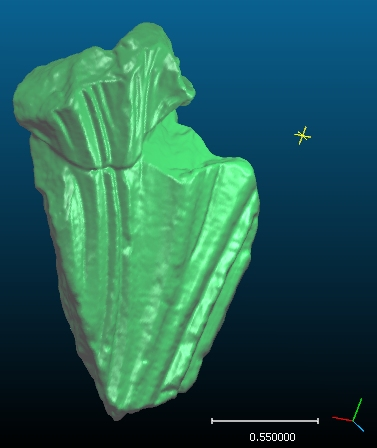
\includegraphics[width=0.3\textwidth]{Partie3_Fonctions/customLight.jpg}
\caption{\label{fig:customLight}Source lumineuse secondaire (\emph{custom light})}
\end{center}
\end{figure}

\par
Il est possible de la d�placer en maintenant enfonc� la touche CTRL tout en faisant un
"PAN" avec la souris (bouton droit enfonc�).
\\
\par
Remarques :
\begin{itemize}
\item \textcolor[rgb]{1.00,0.00,0.00}{Raccourci clavier : F7}
\item L'�toile n'apparait qu'avec la projection orthographique
(voir section~\ref{subsection:centeredPerspective} ou \ref{subsection:viewerPerspective}).
\item L'�toile peut �tre parfois positionn�e initialement � l'int�rieur de l'objet !
\end{itemize}
